\section{Indefinite Integrals}\label{sec:IndefInt}

In this section we focus on computing indefinite integrals.
The process of finding the indefinite integral is called \dfont{integration} (or \dfont{integrating $f(x)$}).

\begin{example}{Indefinite Integral}{IndefiniteIntegral}
Evaluate the following indefinite integral:
$$\int x^5+3x-2\,dx.$$
\vspace{-0.5cm}
\end{example}

\begin{solution} 
Since this is asking for the most general anti-derivative we have:
$$\int x^5+3x-2\,dx=\frac{x^6}{6}+\frac{3x^2}{2}-2x+C$$
where $C$ is a constant.
\end{solution}

{\bf Common mistakes:}
One habit students make with integrals is to \ifont{drop the dx} at the end of the integral.
This is required! Think of the integral as a set of parenthesis.
Both are required so it is clear where the integrand ends and what variable you are integrating with respect to.

Another common mistake is to \ifont{forget the +C} for indefinite integrals.

Note that we don't have properties to deal with products or quotients of functions, that is,
%Just like with derivatives, the following will \dfont{NOT} work:
$$\int f(x)\cdot g(x)\,dx\neq \int f(x)\,dx\int g(x)\,dx.$$
$$\int \frac{f(x)}{g(x)}\,dx\neq \frac{\int f(x)\,dx}{\int g(x)\,dx}.$$
With derivatives, we had the product and quotient rules to deal with these cases.
For integrals, we have no such rules, but we will learn a variety of different techniques to deal with these cases.

The following integral rules can be proved by taking the derivative of the functions on the right side.

\begin{formulabox}[Integral Rules]
Some properties and rules to know:\\
$$\mbox{Constant Rule:}\quad\int k\,dx=kx+C.$$
$$\mbox{Constant Multiple Rule:}\quad\int kf(x)\,dx=k\int f(x)\,dx,\quad\mbox{$k$ is constant}.$$
$$\mbox{Sum/Difference Rule:}\quad\int f(x)\pm g(x)\,dx=\int f(x)\,dx\pm\int g(x)\,dx.$$
$$\mbox{Power Rule:}\quad\int x^n\,dx=\frac{x^{n+1}}{n+1}+C,\quad n\neq -1.$$
$$\mbox{Log Rule:}\quad\int \frac{1}{x}\,dx=\ln|x|+C,\quad x\neq 0.$$
$$\mbox{Exponent Rule:}\quad\int a^{kx}=\frac{a^{kx}}{k\ln a}+C,\quad x\neq 0.$$
$$\mbox{Sine Rule:}\quad\int \sin x\,dx=-\cos x+C.$$
$$\mbox{Cosine Rule:}\quad\int \cos x\,dx=\sin x+C.$$
\end{formulabox}

\begin{example}{Indefinite Integral}{IndefiniteIntegral2}
If $f'(x)=x^4+2x-8\sin x$ then what is $f(x)$?
\end{example}

\begin{solution} 
The answer is:
$$\begin{array}{rcl}
\ds{f(x)=\int f'(x)\,dx}&=&\ds{\int \left(x^4+2x-8\sin x\right)\,dx}\\
\\
&=&\ds{ \int x^4 \,dx + 2\int x\,dx -8 \int \sin x\,dx }\\
\\
&=&\ds{\frac{x^5}{5}+x^2+8\cos x+C,}\\
\end{array}$$
where $C$ is a constant.
\end{solution}

\begin{example}{Indefinite Integral}{IndefiniteIntegral3}
Find the general indefinite integral of $\ds\int 3x^2\,dx$.
\end{example}
\begin{solution}
	$$\begin{array}{rcl}
	\ds{\int 3x^2\,dx} & = & \ds{3\int x^2\,dx}\\
	\\
	&=&\ds{3\frac{x^3}{3}+C}\\
	\\
	&=&x^3+C\\
	\end{array} $$
\end{solution}

\begin{example}{Indefinite Integral}{IndefiniteIntegral4}
Find the general indefinite integral of $\ds\int \frac{2}{\sqrt x}\,dx$.
\end{example}
\begin{solution}
	$$\begin{array}{rcl}
	\ds{\int \frac{2}{\sqrt x}\,dx} & = & \ds{2\int x^{-\frac{1}{2}}\,dx}\\
	\\
	&=&\ds{2\frac{x^{-\frac{1}{2}+1}}{-\frac{1}{2}+1}+C}\\
	\\
	&=&4\sqrt x+C\\
	\end{array}$$
\end{solution}

\begin{example}{Indefinite Integral}{IndefiniteIntegral5}
Find the general indefinite integral of $\ds\int \left(\frac{1}{x}+e^{7x}+x^\pi+7\right)\,dx$.
\end{example}
\begin{solution}
	$$\begin{array}{rcl}
	\ds{\int \left(\frac{1}{x}+e^{7x}+x^\pi+7\right)\,dx} & = & \ds{\int \frac{1}{x}\,dx+\int e^{7x}\,dx+\int x^\pi\,dx+\int 7\,dx}\\
	\\
	&=& \ds{\ln|x|+\frac{1}{7}e^{7x}+\frac{x^{\pi+1}}{\pi+1}+7x+C}\\
	\end{array}$$
\end{solution}

\subsection*{Differential Equations}
An equation involving derivatives where we want to solve for the original function is called a \dfont{differential equation}.
For example, $f'(x)=2x$ is a differential equation with general solution $f(x)=x^2+C$.
Some solutions (i.e., particular values of $C$) are shown below.
$$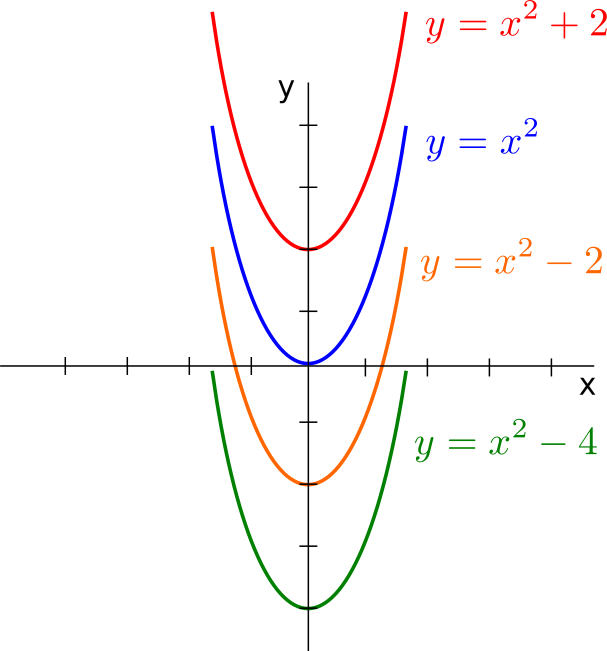
\includegraphics[width=3in]{images2/integral-curves}$$
As seen with integral curves, we may have an infinite family of solutions satisfying the differential equation.
However, if we were given a point (called an \ifont{initial value}) on the curve then we could determine $f(x)$ completely.
Such a problem is known as an \ifont{initial value problem}.

\begin{example}{Initial Value Problem}{Initial Value Problem}
If $f'(x)=2x$ and $f(0)=2$ then determine $f(x)$.
\end{example}

\begin{solution} 
As previously stated, we have a solution of:
$$f(x)=x^2+C.$$
But $f(0)=2$ implies:
$$2=0^2+C\quad\to\quad C=2.$$
Therefore, $f(x)=x^2+2$ is the solution to the initial value problem.
\end{solution}



%
%\dfont{Rectlinear Motion:} We can use the concept of anti-derivatives to find position functions when given the velocity function (or velocity functions when given the acceleration).
%In particular, since $a(t)=v'(t)$ and $v(t)=s'(t)$, where $s(t)$, $v(t)$ and $a(t)$ are the position, velocity and acceleration functions respectively, we have,
%$$v(t)=\int a(t) \,dt,\quad s(t)=\int v(t) \,dt.$$
%
%\begin{example}
%A particle moves along a straight line with acceleration $a(t)=6t+4$. 
%Its initial velocity is $v(0)=-6$ cm/s and initial position is $s(0)=9$ cm. 
%Find $s(t)$.
%\end{example}
%
%\begin{solution}
%Antidifferentiation gives (since $v(t)=\int a(t) \,dt$):
%\[ v(t) = 6 \frac{t^2}{2}+ 4t +C = 3t^2+4t+C.\]
%But $v(0)=-6$, so $C=-6$, and 
%\[ v(t) =  3t^2+4t-6 \]
%Now antidifferentiation again gives  (since $s(t)=\int v(t) \,dt$):
%\[ s(t) = 3 \frac{t^3}{3} + 4 \frac{t^2}{2} -6t +D = t^3+2t^2-6t+D.\]
%But $s(0)=9$, so $D=9$, and we finally get:
%\[ s(t) = t^3+2t^2-6t+9.\]
%\end{solution}


%%%%%%%%%%%%%%%%%%%%%%%%%%%%%%%%%%%%%%%%%%%%%%%%%
\Opensolutionfile{solutions}[ex]
\section*{Exercises for Section \ref{sec:IndefInt}}

\begin{enumialphparenastyle}

Find the antiderivatives of the functions:

%%%%%%%%%%
\begin{ex}
 $\ds 8\sqrt{x}$
\begin{sol}
 $\ds (16/3)x^{3/2}+C$
\end{sol}
\end{ex}

%%%%%%%%%%
\begin{ex}
 $\ds 3t^2+1$
\begin{sol}
 $\ds t^3+t+C$
\end{sol}
\end{ex}

%%%%%%%%%%
\begin{ex}
 $\ds 4/\sqrt{x}$
\begin{sol}
 $\ds 8\sqrt{x}+C$
\end{sol}
\end{ex}

%%%%%%%%%%
\begin{ex}
 $\ds 2/z^2$
\begin{sol}
 $-2/z+C$
\end{sol}
\end{ex}

%%%%%%%%%%
\begin{ex}
 $\ds 7s^{-1}$
\begin{sol}
 $7\ln s+C$
\end{sol}
\end{ex}

%%%%%%%%%%
\begin{ex}
 $\ds (5x+1)^2$
\begin{sol}
 $\ds (5x+1)^3/15+C$
\end{sol}
\end{ex}

%%%%%%%%%%
\begin{ex}
 $\ds (x-6)^2$
\begin{sol}
 $\ds (x-6)^3/3+C$
\end{sol}
\end{ex}

%%%%%%%%%%
\begin{ex}
 $\ds x^{3/2}$
\begin{sol}
 $\ds 2x^{5/2}/5+C$
\end{sol}
\end{ex}

%%%%%%%%%%
\begin{ex}
 $\ds {2\over x\sqrt x}$
\begin{sol}
 $\ds -4/\sqrt{x}+C$
\end{sol}
\end{ex}

%%%%%%%%%%
\begin{ex}
 $\ds |2t-4|$
\begin{sol}
 $\ds 4t-t^2+C$, $t<2$; $\ds t^2-4t+8+C$, $t\ge 2$
\end{sol}
\end{ex}

\end{enumialphparenastyle}
